\section{Dynamische Views}
\label{dv-main}
Mit dynamischen Views sind Seiten einer Anwendung gemeint, deren Inhalt sich zur Laufzeit aufgrund von Nutzerinteraktionen ändert. In AngularJS wird solch ein dynamisches Verhalten über das in Kapitel \ref{frameworks} beschriebene Two-Way-Databinding realisiert. Dieses Konzept ermöglicht das automatische Synchronisieren von Views und Models. Durch das Verändern von Eigenschaften in einem Model ändert sich die Anzeige in der View. Umgekehrt werden Änderungen in der View, beispielsweise durch Benutzereingaben, automatisch ins Model übertragen. Die View ist somit eine Projektion der Daten im Model (Abbildung \ref{angularjs-two-way-databinding}). Physisch gesehen bilden beide jedoch gekapselte Komponenten. Dies fördert zum einen die Testbarkeit und zum anderen die Komponentenbildung\cite{AngularJSDataBinding}. Um diese Synchronisation zu realisieren, wendet AngularJS bestimmte Techniken an, die einen Overhead erzeugen können. Dies führt dazu, dass sich bei zu intensiver Nutzung des Two-Way-Databinding das Antwortzeitverhalten der Anwendung in bestimmten Situationen verschlechtert. Aus diesem Grund werden im Folgenden Herangehensweisen betrachtet, wie dynamische Views möglichst effizient implementiert werden können. Doch dazu ist es zunächst notwendig, die Technik hinter diesem Konzept näher zu betrachten.
\begin{figure}[h]
	\centering
	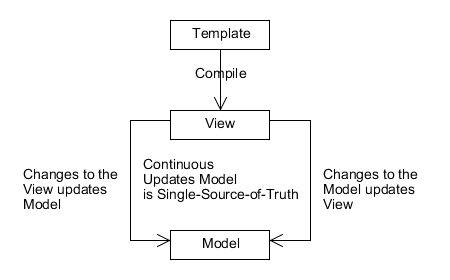
\includegraphics[scale=0.5]{Bilder/Two_Way_Data_Binding.png}
	\caption{AngularJS Two-Way-Databinding}
	\label{angularjs-two-way-databinding}
\end{figure}
In der Theorie kann ein Two-Way-Databinding derzeit auf zwei verschiedene Arten implementiert werden\cite{SBDataBinding}. Die erste Herangehensweise arbeitet mit Gettern und Settern und basiert auf dem Observer-Pattern. Eine Änderung an einem JavaScript-Objekt wird dabei nur über eine entsprechende Setter-Methode durchgeführt. Registrierte Observer können dadurch bei Änderungen über diese Methode benachrichtigt werden. Die zweite Herangehensweise basiert hingegen auf externem Monitoring, auch \glqq Dirty-Checking\grqq{} genannt. Diese Variante wird in AngularJS angewendet. Auch hier registrieren sich Observer, um über Änderungen an einem Objekt informiert zu werden. Die Prüfung, ob sich ein Wert geändert hat, erfolgt jedoch nicht im Objekt selbst, sondern in einem externen Prüfmechanismus. Zu bestimmten Zeitpunkten wird dieser Mechanismus ausgeführt. Dabei werden alle beobachteten Eigenschaften auf Änderungen überprüft. In AngularJS wird dieser Mechanismus in einer Methode namens \emph{\$digest()} durchgeführt und trägt daher den Namen \$digest-Zyklus \cite{SBDataBinding}. Über die Methode \emph{\$watch()} registrieren sich Observer, um Eigenschaften zu überwachen. In der Regel werden Eigenschaften eines Models überwacht. In AngularJS trägt ein entsprechendes Model den Namen \emph{\$scope}. Unterschiedliche, in einem \gls{html}-Template platzierte Direktiven, erzeugen automatisch solch ein Model. Dadurch entsteht eine Hierarchie von Objekten entlang der \gls{html} Struktur \cite{AJSScopes}. Jedes dieser Modelle besitzt eine eigene \emph{\$watch}, \emph{\$digest} und \emph{\$apply} Methode. Die Methode \emph{\$digest} löst dabei den Prüfmechanismus für sich selbst und seine Kind-Elemente aus. Die Methode \emph{\$apply} hingegen löst den Prüfmechanismus für das in der Hierarchie oberste Model aus und ist somit langsamer. \cite{PSApplyDigest}
\\\\
Generell ruft AngularJS die Methode \emph{\$apply} automatisch auf, wenn über entsprechende Direktiven wie \emph{ngClick} auf Nutzerinteraktionen reagiert wurde. Gerade dies ist ein kritischer Zeitpunkt, da Nutzerinteraktionen meist Animationen oder Änderungen an dem \gls{ui} zur Folge haben. Aufgrund dieser Vorgehensweise lässt sich die Problematik bei dynamischen Views in AngularJS ableiten. Je mehr Eigenschaften über ein Two-Way-Databinding beobachtet werden, desto länger dauert das externe Monitoring. Flüssige Animationen oder Änderungen an dem \gls{ui} können dadurch beeinträchtigt werden. Das Ziel ist es daher, die Anzahl der zur selben Zeit beobachteten Eigenschaften zu minimieren.

\subsection{One-Time Bindings und weitere Optimierungsansätze}
\label{dyn-views-onetimebinding}
Um die Durchführung des Prüfvorgangs zu beschleunigen, muss die Anzahl der beobachteten Eigenschaften minimiert werden. Ein erster Schritt in diese Richtung ist das Betrachten der Daten. Man kann Daten an dieser Stelle in statische und dynamische Daten unterteilen. Statische Daten sind Informationen, die sich zur Lebenszeit einer View nicht ändern. Sie dienen als reine Informationsquelle für den Anwender. Dynamische Daten hingegen können sich durch Interaktionen des Anwenders mit der View oder durch andere Ereignisse ändern. Aufgrund dieser Eigenschaft ist ein Two-Way-Databinding für statische Daten überflüssig. Das Beobachten dieser Daten bremst den Prüfvorgang unnötig aus. Zur Optimierung einer View mit vielen statischen Daten ist es demnach sinnvoll, das Two-Way-Databinding für diese Daten zu entfernen. 
\\\\
Das Konzept für diese Umsetzung nennt sich One-Time-Binding. Die Eigenschaften werden dabei weiterhin über AngularJS beobachtet. Jedoch nur so lange, bis die Daten einmalig in der View angezeigt wurden. Im Anschluss wird die Beobachtung entfernt und die folgenden Prüfvorgänge nicht länger beeinflusst. Der Vorteil ist, dass weiterhin die AngularJS-Syntax im \gls{Template} verwendet werden kann und trotzdem die Performance verbessert wird. AngularJS unterstützt ab Version 1.3 nativ eine Syntax für One-Time Bindings \cite{AJSOneTimeBinding}. Listing \ref{dv-ajsonetimebinding} zeigt dessen Verwendung für eine einfache Bücherliste. Entscheidend dabei sind zwei Doppelpunkte zu Beginn einer AngularJS \gls{AJSExpression}. Bei der Verwendung von AngularJS mit einer älteren Version kann die Library Bindonce eingesetzt werden \cite{Bindonce}. Bindonce verwendet das gleiche Prinzip, jedoch müssen Daten in entsprechende Direktiven gekapselt werden, was die Anwendung umständlicher macht. 
\begin{lstlisting}[language=HTML,style=ionicHtmlStyle,caption={Dynamische Views, One-Time Binding mit AngularJS}\label{dv-ajsonetimebinding}]
<ion-item class="..." ng-repeat="book in books">
	<img ng-src="{{::book.image}}"></img>
	<h2 ng-class="::{stock: book.onStock > 0}">
		{{::book.name}}
	</h2>
	<h3>{{::book.author}}</h3>
	<p>{{::book.description}}</p>
	<p style="...">{{::book.price}}</p>
</ion-item>
\end{lstlisting}
Befinden sich viele dynamische Daten in einer View, ist die Optimierung nicht ganz so einfach. Dennoch gibt es auch hier verschiedene Möglichkeiten, eine Optimierung durchzuführen. Generell gilt es, die Anzahl der \gls{dom}-Elemente, die sich zur selben Zeit in einer View befinden, zu minimieren. Wie in Abschnitt \ref{browser-engines} festgestellt, hat dies einen positiven Effekt auf die Performance. Das gilt vor allem für \gls{dom}-Elemente, die vom Two-Way-Databinding betroffen sind. 
\\\\
Ein klassisches Verfahren, um die Anzahl vom \gls{dom}-Elementen in einer View zu verringern, ist der Einsatz von aufklappbaren Bereichen. Der Inhalt dieser Bereiche kann beim Aufklappen in den \gls{dom} eingefügt werden und beeinflusst erst ab diesem Zeitpunkt die Performance. Alternativ können Inhalte auf Detail-Seiten ausgelagert werden, um die Komplexität einzelner Seiten zu verringern. Bei Listen empfiehlt sich der Einsatz von Techniken wie \gls{vs}. Eine nähere Betrachtung dieser Technik findet in Abschnitt \ref{lists-main} statt.
\\\\
Eine weitere Optimierung bei dynamischen Daten kann durch die Begrenzung des Prüfvorgangs auf lokale Models erreicht werden. Wie zuvor beschrieben, besitzt jedes Model die Methode \emph{\$apply}, um den Prüfvorgang für die gesamte Model-Hierarchie durchzuführen. Bei Änderungen, die sich ausschließlich auf die lokale View beziehen, ist dies ein unnötiger Overhead. Mittels eigens definierter Direktiven kann solch ein Verhalten für alle Nutzerinteraktionen implementiert werden. Je größer und komplexer eine Anwendung ist, desto effektiver ist diese Herangehensweise.

\subsection{Analyse des Optimierungspotentials}
\label{dv-analyse}

In diesem Abschnitt wird der Einfluss des Two-Way-Databindings und das Optimierungspotential durch One-Time Bindings auf das Antwortzeitverhalten untersucht. Dabei gilt es Richtwerte zu ermitteln, ab denen eine Optimierung sinnvoll bzw. erforderlich ist. 
\\\\
Zu diesem Zweck wird gemessen, wie viel Zeit ein Prüfvorgang bei einer unterschiedlichen Anzahl von beobachteten Werten in Anspruch nimmt. Entsprechend der Struktur der Testanwendung in Abschnitt \ref{struktur-testanwendung} werden für diesen Testfall zwei Module angelegt. Jeweils eins für die Messung mit One-Time Bindings und eins für Two-Way-Databindings. Für die Laufzeitmessung befindet sich eine Liste mit Beispieldaten in der View. Im oberen Teil kann über ein Eingabefeld die Anzahl der Elemente eingegeben und die Liste damit befüllt werden. Anschließend wird die Laufzeit des Prüfvorgangs für diese View über BenchmarkJS ermittelt und ausgegeben (Listing \ref{dv-benchjs}). Bei den Beispieldaten handelt es sich um eine einfache Bücherliste mit einem Bild, dem Titel, den Autoren, der Beschreibung, dem Preis und der Verfügbarkeit. Wenn das Buch lieferbar ist, wird über \gls{css} der Titel grün hinterlegt. Insgesamt werden durch dieses Template für jedes Buch der Liste sechs Eigenschaften beobachtet. 
\begin{lstlisting}[caption={Dynamische Views, Laufzeitmessung mit BenchmarkJS}\label{dv-benchjs}]
function calculate($scope, callback) {
	var bench = new Benchmark('', {
		'fn': function() {
			this.injectedScope().$digest();
		},
		'onComplete': function() {
			callback(this.stats.mean * 1000)
		}
	});
	Benchmark.prototype.injectedScope = function() { 
		return $scope; 
	};
	bench.run();
}
\end{lstlisting}
Insgesamt wird die Laufzeit pro Variante für sechs unterschiedlich große Mengen von Elementen gemessen. Die ersten fünf entsprechen dabei realistischen Listengrößen auf mobilen Geräten. Die letzte Größe soll als Abgrenzung dienen. Die Messergebnisse sind in Abbildung \ref{dynamischeViews-measurement} aufgeführt. 
\begin{figure}[h]
	\centering
	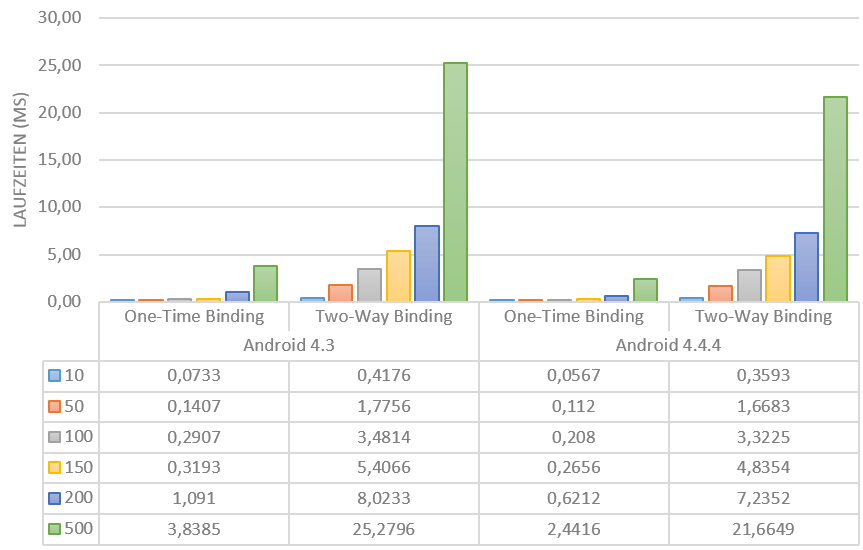
\includegraphics[scale=0.6]{Bilder/Diagramme/DynamischeViews.png}
	\caption{Dynamische Views - Laufzeitmessung One-Time Binding vs. Two-Way-Databinding}
	\label{dynamischeViews-measurement}
\end{figure}
Die Ergebnisse zeigen deutlich, dass One-Time Bindings die Durchlaufzeit eines \emph{\$digest}-Zyklus je nach Anzahl der beobachteten Werte um bis zu 1721\% beschleunigen kann. Im Vergleich zwischen Android 4.3 und 4.4.4 ergeben sich ähnliche Ergebnisse, wobei Android 4.3 im Mittel 41\% langsamer ist. In Abschnitt \ref{performance-ziele} wurde beschrieben, dass für 60 \gls{fps} auf einem mobilen Gerät etwa 10ms zur Verfügung stehen. In dieser Zeit muss die JavaScript-Ausführung sowie der Rendering-Prozess durchgeführt werden. Bereits bei 50 Listenelementen bzw. 300 beobachteten Werten nimmt der \emph{\$digest}-Zyklus bei Android 4.4.4 etwa 17\% der Zeit für ein Frame ein. Abhängig von sonstigen Abläufen kann es dabei bereits zu merklichen Verzögerungen in der Anzeige kommen. Es lohnt sich demnach bereits bei 50 oder weniger Listenelementen eine Optimierung durch One-Time Bindings durchzuführen. Dies gilt aufgrund des geringen Aufwandes insbesondere für AngularJS ab der Version 1.3. 